%Le plan de recherche est à soumettre aux membres du jury et à l'EDPY au plus tard deux semaines avant l'examen.
%La page de couverture dûment signée par le doctorant et le directeur de thèse (et co-directeur si applicable)
%doit être soumise à l’EDPY au plus tard le jour de l'examen.
%The research plan shall be submitted to the jury members and EDPY at the latest two weeks before the candidacy exam.
%The cover page duly signed by the PhD student and the thesis advisor (and co-advisor if applicable) shall be submitted 
%to EDPY at the latest on the day of the exam.

\documentclass[11pt,titlepage]{article}

\usepackage[french,american]{babel}
\usepackage[utf8]{inputenc}
\usepackage[T1]{fontenc}
\usepackage{lmodern}
\usepackage{amsmath,amsfonts,amssymb}
\usepackage{graphicx}
\usepackage{geometry}                % See geometry.pdf to learn the layout options. There are lots.
\geometry{letterpaper}                   % ... or a4paper or a5paper or ... 
%\geometry{landscape}                % Activate for for rotated page geometry
%\usepackage[parfill]{parskip}    % Activate to begin paragraphs with an empty line rather than an indent
\usepackage{graphicx}
\usepackage{amssymb}
\usepackage{epstopdf}
\usepackage{color}
\usepackage[tt]{titlepic}
\usepackage{fancyhdr}
\usepackage{float}
\usepackage{caption}
\usepackage{subcaption}
\usepackage[bottom]{footmisc}
\usepackage{cite}
\usepackage{pdfpages}
\usepackage{braket}
\usepackage{lipsum}
\usepackage{amsmath,amsfonts}
\usepackage{listings}
\usepackage{float}
\usepackage{amsthm}
\usepackage{graphicx}
\usepackage{bm}
\usepackage{algorithm}
\usepackage{algpseudocode}
%\newtheorem{remark}{Remark}
\newtheorem{theorem}{Theorem}
\newtheorem{assumption}{Assumption}
\newtheorem{definition}{Definition}
\newtheorem{proposition}{Proposition}
\newtheorem{corollary}{Corollary}
\usepackage{color} %red, green, blue, yellow, cyan, magenta, black, white
\definecolor{mygreen}{RGB}{28,172,0} % color values Red, Green, Blue
\definecolor{mylilas}{RGB}{170,55,241}
\usepackage{xargs}                      % Use more than one optional parameter in a new commands
\usepackage[pdftex,dvipsnames]{xcolor}  % Coloured text etc.
% 
%\usepackage[english]{babel}
%\usepackage[utf8x]{inputenc}
%% Sets page size and margins
\newcommand{\R}{\mathbb{R}}
\newcommand{\uu}{\mathbf{u}}
\newcommand{\vvh}{\mathbf{v}_h}
\newcommand{\uuh}{\mathbf{u}_h}
\newcommand{\xx}{\mathbf{x}}
\newcommand{\dt}{\Delta t}
\newcommand{\fo}{\bm{\mathcal{F}}}
\newcommand{\Dt}{D_{\Delta t}}
\newcommand{\VV}{\mathbf{V}}
\newcommand{\CC}{\mathbf{C}}
\newcommand{\XX}{\mathbf{X}}
\newcommand{\lv}{\left \vert}
\newcommand{\rv}{\right \vert}
\newcommand{\lno}{\left \Vert}
\newcommand{\rno}{\right \Vert}
\newcommand{\pil}{\pi_\ell}
\newcommand{\pim}{\pi_{\ell-1}}
\newcommand{\vv}{\mathbf{v}}
\newcommand{\LL}{\mathbf{L}}
\newcommand{\TODO}[1]{\color{red}{TODO: #1}\color{black}}
\newcommand{\comm}[1]{\color{blue}{COMMENT: #1}\color{black}}
\newcommand{\E}{\mathbb{E}}
\newcommand{\eff}{\mathcal{F}}
\newcommand{\V}{\mathbb{V}}
\newcommand{\te}{\bm{\theta}}
\newcommand{\phib}{\bm{\phi}}
\newcommand{\pot}{\Phi(\te;y)}
\newcommand{\potl}{{\Phi_{\ell-1}(\te;y)}}
\newcommand{\zl}{{Z_{\ell-1}}}
\newcommand{\zm}{{Z_{\ell}}}
\newcommand{\potm}{{\Phi_{\ell}(\te;y)}}
\newcommand{\dhell}{d_\text{Hell}}
\newcommand{\potp}{\Phi(\te;y')}
\newcommand{\work}{\mathcal{W}}
\newcommand{\QoI}{\text{QoI}}
\newcommand{\HH}{\mathbf{H}}
\newcommand{\sig}{\bm{\sigma}}
\newcommand{\nel}{N_\text{el}}
\newcommand{\ff}{\mathbf{f}}

\newcommand{\del}{\nabla}
%% Useful packages
\usepackage{amsmath}
\usepackage{graphicx}
\usepackage[colorinlistoftodos]{todonotes}
\usepackage[colorlinks=true, allcolors=blue]{hyperref}
%\usepackage{algpseudocode}
%\usepackage[ruled,vlined]{algorithm2e}
%\SetKwFunction{MH}{Metropolis-Hastings}% 
%======================= Titlepage =========================================================
%-------------------------------------------------------------------------------------------------------------------------------------------------------
\titlepic{
\includegraphics[width=17cm]{figures/edpy_header}}

\title{\textbf{Research Plan}\\ \vspace*{0.5cm}\large{\textbf{Titre provisoire de la thèse / Provisional thesis title}}}

\author{Candidate: Juan Pablo Madrigal Cianci\vspace*{1cm}\\Advisor: Fabio Nobile }
\date{\today}				%activate to remove date
%========================================================================================

\newcommand{\ham}{\hat{\mathcal{H}}}

\begin{document}
%========================  Top header ======================================================
\pagestyle{fancy} \pagenumbering{arabic} \setcounter{page}{1}
\addtolength{\headheight}{\baselineskip}
\newcommand{\ffont}{\fontsize{8}{8}\selectfont}
%\lhead{\textit{DOCTORAL SCHOOL}}
\lhead{\textit{DOCTORAL PROGRAM IN MATHEMATICS}}
\rhead{\bfseries\ffont  
\includegraphics[width=55pt]{figures/epfl_logo.pdf}}
\renewcommand{\headrulewidth}{0.4pt}

%=========================================================================================

%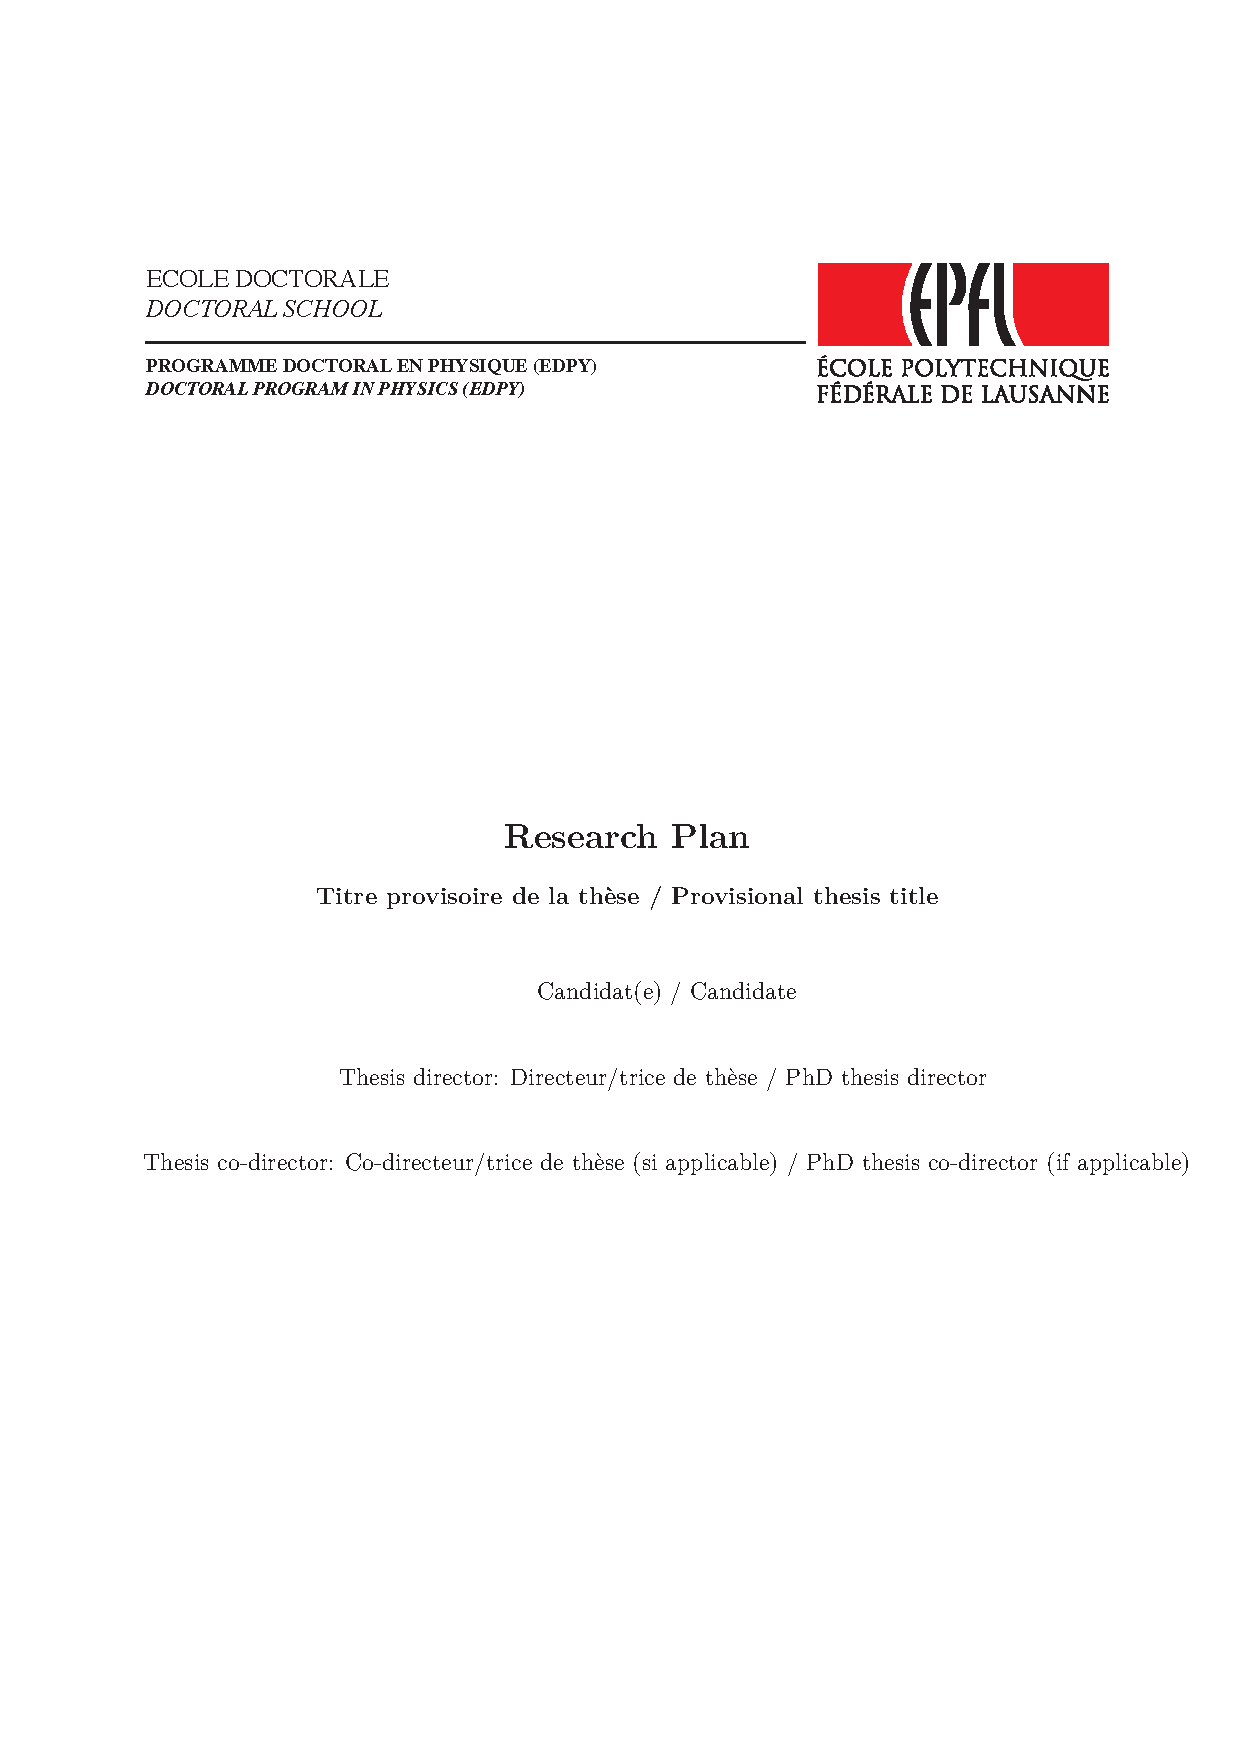
\includepdf[pages=-]{cover.pdf} % please uncomment this to include cover.pdf
\pagenumbering{gobble}
\maketitle  % please uncomment this to compile the title page
\newpage
\tableofcontents
\newpage
\hspace*{0.3cm}
\section{Introduction, Setup, and  Objectives}
\pagenumbering{arabic}
% 1.	Introduction (cadre général) / Introduction (general framework): 1 page

\hspace*{0.3cm}

% 1.	Introduction (cadre général) / Introduction (general framework): 1 page

\hspace*{0.3cm}
\color{red}  ALMOST FINAL DRAFT  \color{black}
\subsection{Introduction}
This thesis project focuses on the development and implementation of Markov Chain Monte Carlo (MCMC) techniques, as well as their multi-level and multi-index extensions (MLMCMC and MIMCMC respectively) techniques for Bayesian inverse problems (BIP) arising in seismic
and geophysical applications; such as seismic inversion and earthquake
source estimation. The goal of these type of problems is to determine a set of parameters $\te$, which identify e.g, the earthquake source characteristics, based on few recorded waveforms at the surface. We will use the elasto-dynamic wave  equation to model such seismic event, and will take the recorded waveform to be the time series of the ground displacement\footnote{We remark however that in practice these receiver can also measure  other wave related quantities, such as velocity or acceleration of the ground at the recording position. } at different receivers scattered throughout the surface. In this case, we take the set of unknown parameters $\te$ to be properties related to the source function (location, set-off time, moment tensor), as well as the material properties of the medium, such as density and Lam\'e parameters.  Traditionally, seismic inversion has been performed using a deterministic approach, by introducing a cost functional $J(\te)$ measuring the misfit between the modeled surface waveforms and the observed ones. This cost functional is then minimized using traditional optimization algorithm to find a minimizer (see, e.g, \cite{tromp2005seismic,burstedde2009algorithmic}). In statistical terms, this approach can often be interpreted as a maximum likelihood point estimation. However, there is a growing need to quantify the uncertainty in these methods \cite{SRCMOD}, by adopting, for instance, a Bayesian approach and sampling techniques such as MCMC. The aim of this work is to develop accelerated and efficient MCMC algorithms to tackle this problem.
\subsection{Objectives}
Modern computing facilities and computational techniques are starting to make Bayesian inversion approaches and  MCMC feasible for large scale inverse problems involving partial differential equations (PDEs) \cite{stuart2010inverse}.There is a wealth of literature devoted to those problem arising from elliptic PDEs (see, for example\cite{stuart2010inverse}), however, this is otherwise rather scarce for hyperbolic equations. One of the first objectives from this work is then to extend the BIP theory to cover these type of problems. An additional issue with a MCMC computation is its inherent cost. Contrary to plain Monte Carlo, MCMC is sequential in nature and produces samples that are, in general, correlated. One proposed idea to mitigate this burden is the use of multi-level  samplers \cite{dodwell2015hierarchical,hoang2013complexity,giles2008multilevel}, for which most of the work is done using a coarse discretization of the PDE, and the sample thus obtained is then ``corrected'' using more refined discretization levels. there are few results available so far. This is a rather new approach to MCMC techniques and as such, there are rather few results available so far. A further improvement on the multi-level sampler is offered by the multi-index technique \cite{haji2016multi} there are the multi-index samplers, for which the computational cost can be reduced even further \color{red} by taking different discretization directions. \color{black}.
% In summary, this thesis will cover the following topics, some of which have already been explored and are currently the topic of an upcoming paper (in draft state as of \today). 
%\begin{enumerate}
%	\item Formulation of the BIP and study of its well-possedness for the hyperbolic case.
%	\item Implementation of efficient and addaptive MLMCMC schemes.
%	\item Implementation of efficient and addaptive MIMCMC schemes.
%\end{enumerate}
%and their validation with some well defined case studies in 2 and 3 dimensions. 
\subsection{Problem Set-up}
We are interested in determining  the earthquake properties of a seismic event. Experimentally,  data  $\mathbf{y}\in \R^d$, assumed to be  polluted by some additive random noise $\eta$, is recorded at $N_r$ receivers and at $N_t$ time instances. This receivers can be located, for example, at the surface of the earth or in observation wells.  The recorded data can be described by an observation operator $\mathcal{F}$  applied to a realization of a model for the seismic wave propagation, $\uu:=\uu(\te)$, viewed as a map from a parameter space $\Omega$ to $\R^d$. Based on this, our aim is then to  determine a conditional probability distribution $\pi(\te|y)$  of a set of parameters $\theta\in \Omega$ such that  $\mathcal{F}(\te)=\mathcal{F}(\uu(\te))$ closely resembles the measured data $\bm{y}$.  In the following subsections we will describe in more detail the model used to describe the seismic motion, the observation operator, and the Bayesian inversion procedure used to obtain $\pi(\te|y)$.
\begin{figure}
	\centering
	\includegraphics[width=0.5\linewidth]{setup}
	\caption{Experimental setup of the problem. An earthquake generated at source travels through material properties and the displacement of the earth is recorded at the receivers (purple squares). Based on the recording data of the receivers, we employ MCMC techniques to recover the source location. }
	\label{fig:setup}
\end{figure}

\subsubsection{Forward Problem}

We follow the analysis presented  in \cite{ motamed2013stochastic, motamed2015analysis,kocher2014variational,joly2003variational}. We denote the spatial variable by $\xx$ and the set of unknown parameters by $\te$. Consider an elastic,  non-homogeneous medium in an open, bounded set  $D\subset \R^d$, with $\partial D=\Gamma_D\cup \Gamma_N$, $\Gamma_D\cap \Gamma_N=\emptyset$, $|\Gamma_D|,\ |\Gamma_N|>0$, for $d=2,3$ and a time interval $I=[0,T]$. Given some complete probability space $(\Omega,F,P)$, \color{red} where $\Omega$ is...\color{black} we can pose the following stochastic initial boundary value problem given by \begin{subequations}\label{strongform}
	\begin{align}
	&\varrho(\xx,\te)\uu_{tt}(t,\xx,\te)-\del\cdot\mathbf{\sig}(\uu(t,\xx,\te))=\ff(t,\xx,\te) & \text{in } I\times D\times \Omega\\
	&\uu(0,\xx,\te)=\mathbf{g_1}(\xx), \ \ \uu_t(0,x,\te)=\mathbf{g}_2(\xx) & \text{on } \times D\times \Omega\\
	&\sig(\uu(t,\xx,\te))\cdot\mathbf{n}=\mathbf{0}& \text{on }I\times\Gamma_N\times \Omega,\\
	&\uu(t,\xx,\te)=\bm{0}&\text{ on } I\times\Gamma_D\times \Omega,
	\end{align}
\end{subequations}
where  $\uu: I\times D\times\Omega  \rightarrow\R^d$ $,\xx\in \R^d,\te\in\Omega, t\in I$, and with  $\sig=\lambda(\xx,\te)\del\cdot\uu I +\mu(\xx,\te)(\del\uu+(\del\uu)^T)$. Here we denote by $\uu$  the displacement vector, by $\varrho>0$ the material density, by $\lambda,\mu$ the Lam\'e parameters,  and by $\ff$ a (generalized) body force. \begin{assumption}\label{as:th} \color{red} include comment on assumptions\color{black}
	Let $s\geq 0$ be an integer. We assume that \begin{eqnarray}
	\ff(\cdot,\cdot,\te)\in\LL^2([0,T];\HH^s(D))\text{ for a.e. $\te\in \Omega$}, & \mathbf{g}_1\in \HH^{s+1}(D), &\mathbf{g}_2\in \mathbf{H}^s(D), \ \ s\geq 0.
	\end{eqnarray}
\end{assumption}
\noindent Under Assumption \ref{as:th}, problem (\ref{strongform}) admits a unique solution for a.e $\te \in \Omega$. We can then interpret the solution $\uu(t,\xx,\te)$ as a Banach space-valued function on $\Omega$  \cite{motamed2015analysis}, \begin{equation}\label{eq:wf_s}
\uu=\uu(\te):\Omega\rightarrow\bf{V}:=\mathbf{C}^0([0,T];\HH^{s+1}(D))\cap\mathbf{C}^1([0,T];\HH^s(D))\cap\HH^{2}([0,T];\HH^{s-1}(D)), \ \ s\geq 0.
\end{equation}
In turn, (\ref{eq:wf_s}) is a weak solution to problem (\ref{strongform}) provided that at $t=0$, $\uu(\te)=\mathbf{g}_1,\ \uu_t(\te)=\mathbf{g}_2$ and that for all test functions $\vv\in \mathbf{C}_0^\infty([0,T];H^1(D))$ the following weak formulation holds \begin{eqnarray}
\int_0^T\int_{D}\left(\varrho \uu_{tt}\cdot\vv+\del\vv:\sig(\uu)\right)d\xx dt=\int_0^T\int_{ D}\ff\cdot\vv d\xx dt.
\end{eqnarray}
For the analysis of the well possedness of the Bayesian inverse problem we will need $\uu$ to be Lipschitz in $\Omega$. To this end, we \color{red} quote,recall,...\color{black} the following theorem, presented in \cite{motamed2015analysis}:
\begin{theorem}\label{thm:lips} For the solution of problem (\ref{strongform}) with data given by Assumption \ref{as:th}  \color{red} check on additional assumptions on Motamed's paper \color{black} and with uniformly elliptic material properties,  we have that
	\begin{equation}
	\partial_{\theta_n}\uu(\te)\in\mathbf{C}^0([0,T];\HH^{s}(D)), \ \ s\geq 0,
	\end{equation}
	where $\theta_n$ denotes the $n^\text{th}$ component of $\te$. Moreover, $	\partial_{\theta_n}\uu(\te)$ is uniformly bounded in $\Omega$.
\end{theorem}
\begin{proof}
	The previous theorem is a particular case of Theorem 3 in \cite{motamed2015analysis}, for the case $k=1, $  \color{red} what is k?\color{black}and $s\geq 0$. 
\end{proof}
\begin{corollary}
	Under the assumptions of the previous theorem, $\uu(\te)$ is Lipschitz continuous, when seen as a map from $\Omega$ tp $\mathbf{C}^0([0,T];\HH^{s}(D))$.
\end{corollary}
\noindent For the purpose of this project, system (\ref{strongform}) is approximated numerically, using a spectral element method for the space discretization and the leapfrog method for the time marching scheme. 
\subsubsection{Observation Operator}
for the application at hand, data is gathered using an observation operator. As such, we will also need to study the properties of this operator in order to properly formulate the well possedness of the BIP.  We define the forward map $\fo:\Omega\rightarrow\R^{m\times N_{rec}}$ by  $$\bm{\mathcal{F}(\te)}=(\mathcal{O}_1(\uu(\te)),\dots,\mathcal{O}_{N_{rec}}(\uu(\te)),$$ where $\mathcal{O}_i\in(\mathbf{V}')^m$ is a linear observation operator at times $\{t_1,\dots,t_m \},$ associated to the $i^\text{th}$ receiver. In many problems in seismic inversion, data is only available at discrete points in the spatial domain, which in turn implies that the observation operator lacks enough regularity. To alleviate this, we define our $i^\text{th}$ linear operator as \begin{align}
\mathcal{O}_i(\vv)=\left(\frac{1}{|\mathcal{B}(\xx_i,r)|}\int_{{\mathcal{B}(\xx_i,r)}}\vv(t_1,\xx),\dots,\frac{1}{|\mathcal{B}(\xx_i,r)|}\int_{{\mathcal{B}(\xx_i,r)}}\vv(t_m,\xx)\right)^T,
\end{align} for any $\vv\in C^0([0,T],L^2(D))$, and where $\mathcal{B}(\xx_i,r)$ denotes the ball centered at $\xx_i$ with radius $r$. Let us denote $$\lv \fo (\te)\rv^2=\sum_{i=1}^{N_{rec}}\max_j\lv\mathcal{O}_{i,j}(\uu(\te))\rv^2.$$ 
% $$\Omega \ni\te\rightarrow\mathcal{F}:=(\mathcal{O}_1(\te),\mathcal{O}_2(\te),\dots,\mathcal{O}_{N_\text{obs}}(\te))=(\mathcal{O}_1(\uu(\te)),\mathcal{O}_2(\uu(\te)),\dots,\mathcal{O}_{N_\text{obs}}(\uu(\te))).$$ Here $V^*$ can be, for example \begin{align}
%V^*&=V_1=\LL^2([0,T];\HH^1(D))\cap \HH^1([0,T];\LL^2(D)), \quad \text{ or }\\
%V^*&=V_2=\mathbf{C}^0([0,T];\HH^1(D))\cap \mathbf{C}^1([0,T];\LL^2(D)).
Based on this, we can show that $\fo$ is Lipschitz continuous:
\begin{proposition}\label{prop:bdd_obs} Under the assumption of uniform ellipticity \color{red} define this or state as an assumption\color{black} on the material properties, $\bm{\mathcal{F}}$ is Lipschitz continuous. 	
\end{proposition} \color{red} not too happy with how equation is being displayed\color{black}
\begin{proof}
	We begin by noting that \begin{align}&| \mathcal{O}_{i,j}(\vv)|=
	\lv \frac{1}{|\mathcal{B}(\xx_i,r)|}\int_{\mathcal{B}(\xx_i,r)} \vv(t_j,\xx)d\xx\rv\nonumber \\&\leq \sqrt{ \frac{1}{|\mathcal{B}(\xx_i,r)|}\lno \vv(t_j,\cdot)\rno^2_{L^2(\mathcal{B}(\xx_i,r))}  }\leq \sqrt{ \frac{1}{|\mathcal{B}(\xx_i,r)|}\lno \vv(\te)\rno^2_{C^0([0,T];L^2(\mathcal{B}(\xx_i,r)))}}
	\end{align}
	 This in turn implies that  $\forall\  \te,\te'\in\Omega$, $$|\eff(\te)-\eff(\te')|\leq \Vert \uu(\te)-\uu(\te')\Vert_V.$$
Moreover, by Theorem \ref{thm:lips}, we have that there exist a $C_L>0$ such that $$\Vert \uu(\te)-\uu(\te')\Vert_V\leq C_L\Vert \te-\te'\Vert_{L^2(\Omega)},$$
thus, 
$$ |\eff(\te)-\eff(\te')|\leq C_L\Vert \te-\te'\Vert_{L^2(\Omega)}.$$\end{proof}
\subsubsection{Bayesian Formulation}
We consider a bounded and finite parameter space $\Omega$ \color{red} explain with bounded.\color{black} We will use the assumption of additive noise, i.e, we consider the case where we are given data $y$ polluted by some noise $\eta$, with $\eta,y\in \R^q$ and modeled by some forward map or linear observation operator $\mathcal{F}:\Omega\rightarrow\R^q$ such that
\begin{align}
y=\mathcal{F}(\te)+\eta, \quad \eta\sim g,
\end{align}
 where $f$ is some arbitrary probability distribution. Given the noisy, recorded data $y$, we are interested in determining a set of parameters $\te$ such that when used as input in $\ref{strongform}$, we obtain a wave form that closely resembles the one observed. To do so, we adopt a    Bayesian approach to the problem of determining $\te$ from $y$.  Roughly speaking, contrary to the deterministic counterpart, where only point estimates are obtained, the
Bayesian approach will lead to the notion of finding a probability measure
$\pi^y$ in $\Omega$, containing information about the relative probability of different
states $\te$, given the data y. Incorporating our prior beliefs in a density $\pi^0$ and denoting the conditional probability of $\te$ given $y$, by $\pi^y$, we have that from Bayes theorem \begin{align}
\pi^y\propto g(y-\mathcal{F}(\te))\pi^0(\te),
\end{align}
Moreover, we choose priors $\pi^0$ such that $\pi(\Omega)=1$, that is, the posterior is absolutely continuous with respect to the prior. Using Theorem 6.31 in \cite{stuart2010inverse}, we can rewrite the previous expression in terms of the Radon-Nikodym derivative \begin{align}\label{eq:radon}
\frac{d\pi^y}{d\pi^0}\propto\exp(-\Phi(\theta,y)),
\end{align}
where we are abusing notation and representing both density and distribution with the symbol $\pi$, and where we call $\Phi(\te,y)$ the potential function. For simplicity, we will limit ourselves to the case of additive Gaussian noise case; $$g=\mathcal{N}(0,\Sigma).$$



\newpage
\hspace*{0.3cm}
\color{red}  ALMOST FINAL DRAFT; DON'T KNOW IF I SHOULD INCLUDE A BRIEF DESCRIPTION OF MCMC \color{black}
\section{State of the Art}\label{sec::obj}
% 2.	Objectifs / Objectives: ½ page

\hspace*{0.3cm}

\noindent We now discuss the current state of the art of the research at hand. There are two main points to address in this respect; the first one relates to the current state of seismic source inversion, and the second one addresses the state of  multi-level and multi-index Markov chain Monte Carlo methods. The former has been traditionally dominated by deterministic inversion, with the use of the more robust, MCMC based probabilistic inversion having been recently introduced. The latter tries to extend the ideas of multi-level and multi-index Monte Carlo to an MCMC setting. This in turn is still at a very early stage, with only a handful of papers discussing this ideas.  

 \subsection{Seismic  Inversion}
\color{blue} Some things in this section borrow form the CRG4 grant proposal...How can I cite that? \color{black}
In earthquake  inversion, we try to estimate the material properties (such as velocity, density and Lam\'e parameters) or the kinematic parameters of the earthquake rupture process that occurs on a geological fault plane of finite spatial extent (finite-fault) within the earth. These parameters can be the point-source location, the  spatially variable displacement across the fault surface (slip), the slip direction, the slip duration (which is tied to a poorly known slip-rate function), and the rupture time (time at which each point on the fault starts to slip; this is tied to a rupture velocity). To this end, seismologists have developed numerous techniques over the past decades.  Traditionally, a deterministic approach has been employed, on which a misfit  functional $J(\te)$ (where $\te$ represents the vector of parameters of interest) measuring the difference between some recorded data $y$ and some generated data $\mathcal{F}(\te)$ is defined and minimized. Thus the deterministic inversion reads as a constrained optimization problem $$\min_{\te \in \bm{\Omega}} \Phi(\te)$$ with $$\Phi(\te)=J(\te)-\frac{\alpha}{2}R,\quad \text{such that (\ref{strongform}) holds}, $$  where $R$ is a regularizing term (such as Tykhonov or total variation) and $\alpha$ is  some regularization parameter. This approach has been studied extensively \cite{hormander1985analysis,komatitsch1999introduction} and it is still a fairly active area of research in the geophysics community, however, these methods are prone to discrepancies \cite{beresnev2003uncertainties}. An example can be seen for the 2011 Tohoku earthquake (Japan), where a survey over more than 20 different inversion methods described in various papers  yields widely different results for the source location (see, for example, \cite{hayes2011rapid,shao2011focal,SRCMOD}). This calls for models that can  accurately quantify  uncertainty.\begin{figure}[H]
	\centering
	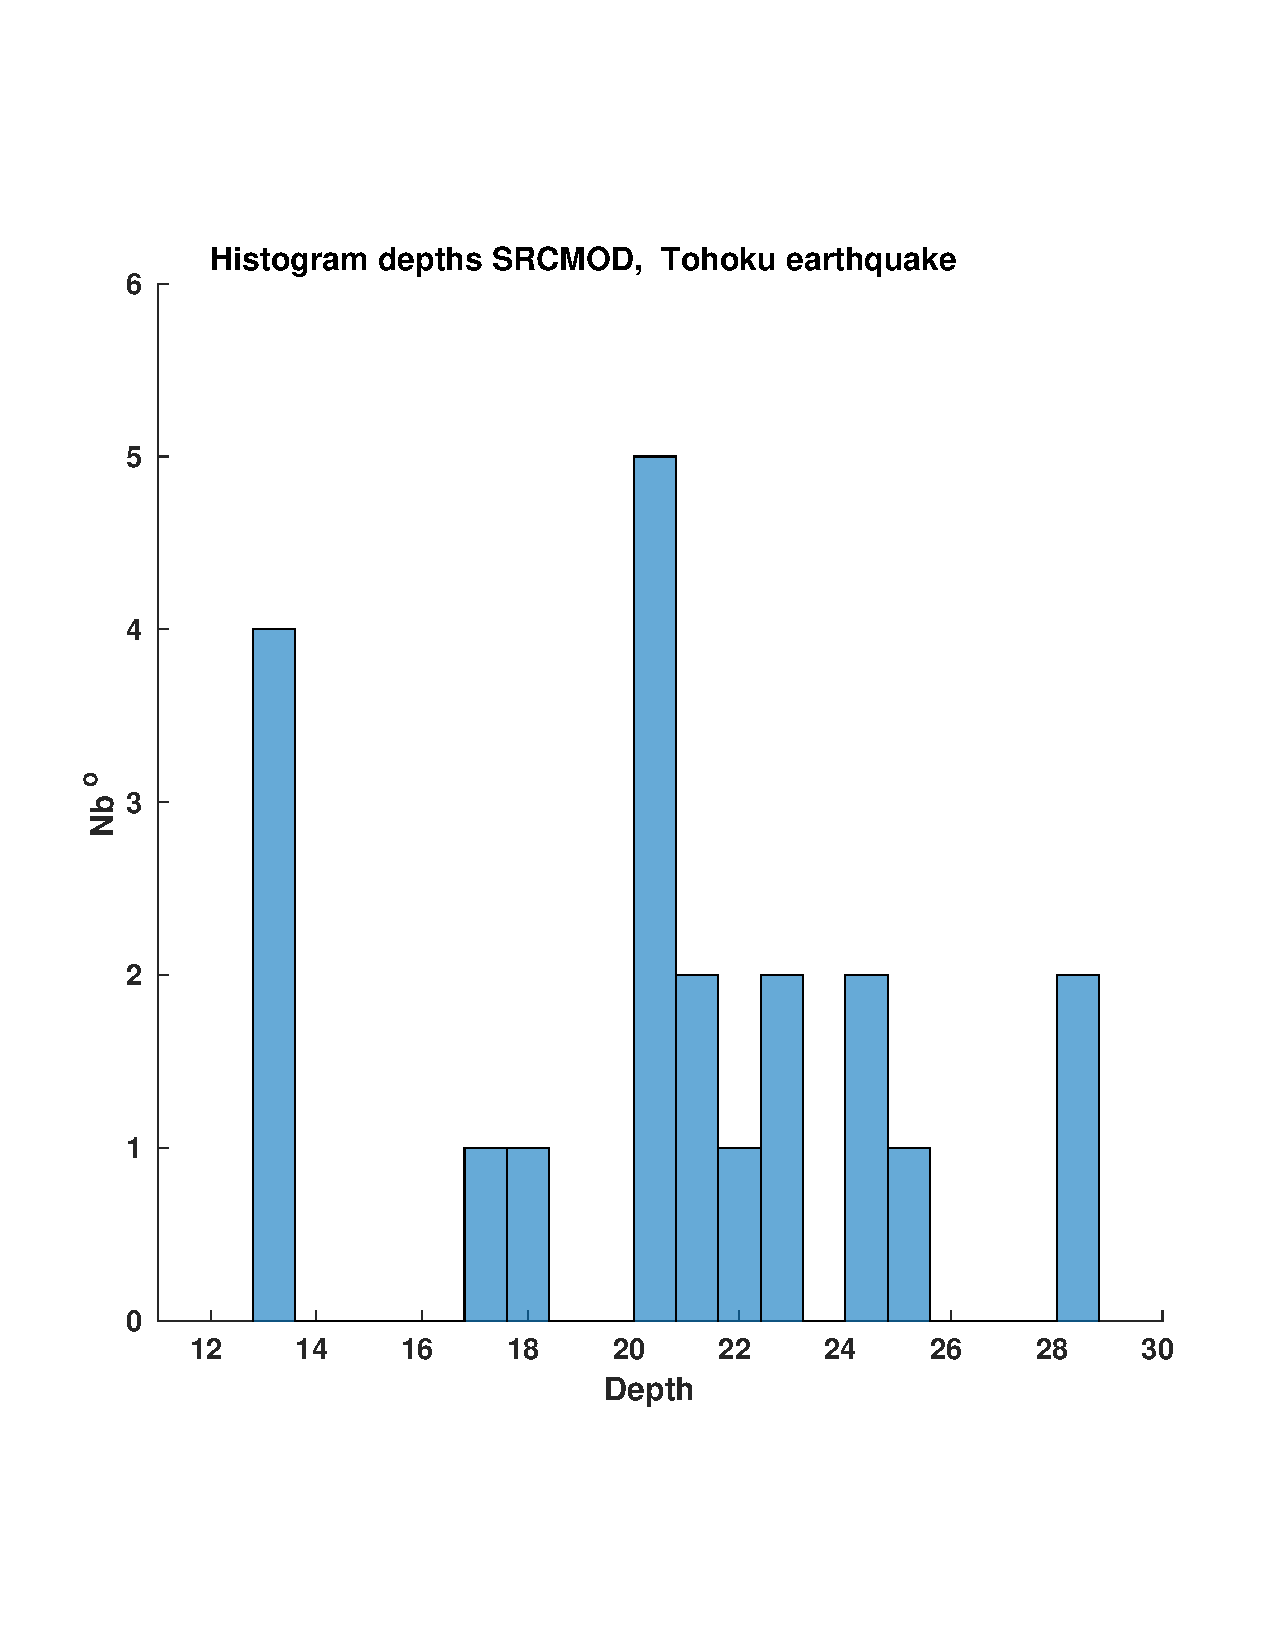
\includegraphics[width=0.5\linewidth]{figures/HistogramTohoku}
	\caption{Histogram of different source locations obtained for the 2011 Mw 9.0 Tohoku earthquake.}
	\label{fig:histogramtohoku}
\end{figure}



 \noindent More recently,  full Bayesian estimation of earthquake  properties has been attempted (see, for example \cite{minson2013bayesian,bui2013computational}) although it is still in its early stages and geared mostly towards inversion on the material properties of the medium, rather than on the physical properties of the earthquake.  This lack of development of this type of methods is mostly linked to the large cost associated to obtaining numerical simulations of the  forward problem of local, regional, or global seismic wave propagation. To mitigate this computational burden, various simplifying assumptions are typically made. Thus, a complete or comprehensive quantification of the uncertainties in the resulting finite-fault rupture models, owing to (a) data errors; (b) unknown earth structure; (c) unknown rupture physics (e.g. detailed fault geometry; poorly known slip-rate function); (d) simplification in computing the response functions is still missing in the literature. 
 
 \subsection{Markov Chain Monte Carlo}

\subsection{Muti-level and Multi-index Markov Chain Monte Carlo}
The work done on ML/MI-MCMC is still on its very early stages, with only a handful of papers on the topic \cite{dodwell2015hierarchical,hoang2013complexity,jasra2018multi} , focusing mostly on inverse problems involving elliptic PDEs. To the best of our knowledge, there has not been a rigorous attempt to extend these methods to inverse problems involving hyperbolic PDEs. Moreover, the algorithms discussed therein are open to improvements. To better understand the theory behind these methods, we first discuss briefly the ideas underlying  MLMC and MIMC, as ML/MI-MCMC are an extension of these to MCMC.  MLMC are algorithms for computing expectations that arise in stochastic simulations in cases in which the stochastic model can not be simulated exactly, rather approximated at different levels of accuracy and as such, at different computational costs. Just as Monte Carlo methods, they rely on repeated random sampling, but these samples are taken on different levels $\ell$ of accuracy (cheap simulations), in such a way that the majority of the samples $M_\ell$ are obtained with low accuracy. In the case of PDE driven inverse problems, this can be understood as introducing a hierarchy of discretizations $\{h_\ell\}_{\ell=0}^L$ such that the cost of solving the PDE and the accuracy of the numerical solution increase as $\ell$ increases. %By following an idea similar to that of multi-grid algorithms, where the majority of the samples are obtained  at  coarser discretizations, 
 MLMC methods can greatly reduce the computational cost of standard Monte Carlo methods by taking most of the samples at a low accuracy and corresponding low cost, and only very few samples  at high accuracy and corresponding high cost.   In the standard MLMC approach we denote the resulting approximation of a quantity of interest using mesh size $h_\ell$ in the simulation of a forward observation  operator event by $\QoI_\ell(\te)$ . Then, the expected value of the finest approximation, $\QoI_L$, can be expressed as
\begin{align*}
%\label{eq:telescoping}
\E[{\QoI_L}] & =
\E[\QoI_0] + \sum_{\ell=1}^L \E[\QoI_{\ell}-\QoI_{\ell-1}],
\end{align*}
and the MLMC estimator is obtained by approximating the expected values
in the telescoping sum by sample averages as
\begin{align}
\label{eq:MLMC_estimator}
\mathcal{A} & = \frac{1}{M_0}\sum_{m=1}^{M_0}\QoI_0(\te_{0,m}) +
\sum_{\ell=1}^L\frac{1}{M_\ell}\sum_{m=1}^{M_\ell}
\left(\QoI_{\ell}(\te_{\ell,m})-\QoI_{\ell-1}(\te_{\ell,m})\right),
\end{align}
where, for every $\ell$,  $\{\te_{\ell,m}\}_{m=1}^{M_\ell}$
denotes independent identically distributed (i.i.d.) realizations of the mesh-independent random variables $\te$. If $W_\ell$ is the average cost associated with generating one sample of the difference, $\QoI_{\ell}-\QoI_{\ell-1}$, or simply $\QoI_0$ if $\ell=0$, then the cost of the
estimator~\eqref{eq:MLMC_estimator} is
\begin{align}
\label{eq:work_sum}
\work & = \sum_{\ell=0}^{L} M_\ell W_\ell.
\end{align}
%
We assume that the work required to generate one sample of mesh size
$h$ is proportional to $h^{-\gamma}d$, where $d$ is the dimension of the
computational domain and $\gamma > 0$ represents the complexity of
generating one sample with respect to the number of degrees of freedom.
Thus, we model the average cost on level $\ell$ as
\begin{align}
\label{eq:wl_model}
W_\ell \leq h_\ell^{-\gamma}d,
\end{align}
and consequently use the representation
\begin{align}
\label{eq:model_work}
\work & \leq \sum_{\ell=0}^{L} \frac{M_\ell}{h_\ell^{\gamma}}
\end{align}
for the total work to evaluate the MLMC estimator~\eqref{eq:MLMC_estimator}.
It can be shown that under certain conditions on the ccuracy of the PDE solver and on the variance of the increments, for a given tolerance $\epsilon$, there exist a constant $c_\text{mlmc}$ \begin{align}\label{mlmc_cost}
\E[\work]\leq\begin{cases}
c_\text{mlmc}\epsilon ^{-2}& \beta>\gamma \\
c_\text{mlmc}\epsilon ^{-2}\log(\epsilon)^2& \beta=\gamma \\
c_\text{mlmc}\epsilon ^{-2-(\gamma-\beta)/\alpha}& \beta<\gamma, \\
\end{cases}
\end{align}
where $\alpha$ is related to the numerical accuracy of the PDE solver and $\beta$ is related to the decay rate of the variance of the increments \cite{giles2008multilevel}. A further improvement over the non-optimal regime ($\beta>\gamma$) can be obtained using  multi-index Monte Carlo (MIMC), for which different discretization directions are used \cite{haji2016multi}. These methods have successfully been implemented for a wide variety of problems, including simulation of random paths, option pricing etc. Extending these methods to a MCMC setting is not a trivial task since (i) the MLMCMC algorithm must be constructed in such a way that  samples in two continuous chains are correlated (so that the variance of the increment in $\QoI_\ell$ decays as $\ell$ increases) and the algorithm should, ideally generate samples with a small autocorrelation time within chains, since, as opposed to pure Monte Carlo, MCMC generates samples that are correlated, which will generate a bias on the estimator.  As mentioned before,  only a few works so far have dealt with the ML-MI extension of MCMC methods for posterior exploration in Bayesian inversion. Of theoretical importance is the work of \cite{hoang2013complexity}, as it provides a very thorough analysis to a particular version of these methods applied to inverse problems involving elliptic PDEs. However, the method described in that paper generates proposals based on independent samplers (see \cite{asmussen2007stochastic}), and this in turn can become widely inefficient if the proposal generating function is not constructed carefully. The work of \cite{dodwell2015hierarchical} proposes a more efficient algorithm and provides an estimate for the total work necessary to obtain a tolerance of $\epsilon$, given by a form similar to (\ref{mlmc_cost}). \begin{definition}
	We define the mean squared error (MSE) associated to a MCMC algorithm by $$e^2_{MSE}(\QoI_{\ell})=\E_\vartheta\left[ \left(\frac{1}{M_\ell}\sum_i^{M_\ell}\QoI^i-\E_\mu(\QoI)\right)^2	\right], $$
	where $\QoI$ is some quantity we wish to estimate, following some (unachievable) distribution $\mu$ and where $\vartheta$ is the distribution from which we are actually able to sample.  \end{definition} 

\begin{definition}
	Suppose each sample at level $\ell$ has an associated cost $\mathcal{W}_\ell$. We denote the $\varepsilon$-cost, i.e, the cost associated to obtaining a mean squared error of $\varepsilon$ when estimating $\QoI$ by $\mathcal{W}_\ell^\epsilon(\QoI).$ 
\end{definition}
\begin{theorem}
Denote by $Y_\ell=$	Suppose that all chain have been sufficiently burned-in and that there exist $\alpha,\beta,\gamma>0$, and $\varepsilon<e^{-1}$, such that $\alpha\geq\min(\beta,\gamma)$. Suppose the following assumptions hold for all $\ell\geq 0 $: \begin{enumerate}
		\item[i)] $\lv \E_{\pi_{\ell,h}}[Q]-\E_{\pi_\ell[Q]}\rv \leq C_1 h_\ell^{\alpha  }$
		\item[ii)] $\V_{\pi_{\ell,h}}[Y_\ell]\leq C_2 h_\ell^{\beta}$
		\item[iii)] $e_\text{MSE}(Y_\ell)\leq C_3 \sup|\V_{\ell}[Y_\ell]|M_\ell^{-1/2}$
		\item[iv)] $W_\ell^\epsilon(\QoI)\leq C_4h_\ell^{-\gamma},$
	\end{enumerate}
	then, there exist a number of levels $L$ and a sequence of $\{N_\ell\}_{\ell=0}^L$ such that $$e(\QoI_{L})\leq\varepsilon,$$ and \begin{align}
	\mathcal{W}_L^\epsilon(\QoI)\leq C_5\begin{cases}
	\varepsilon^{-2}|\log\varepsilon|, & if \ \beta>\gamma,\\
	\varepsilon^{-2}|\log\varepsilon|^3, & if \ \beta=\gamma,\\
	\varepsilon^{-2+(\gamma-\beta)/\alpha}|\log\varepsilon|, & if \ \beta<\gamma.\\
	\end{cases}
	\end{align}
\end{theorem}  




\newpage

\hspace*{0.3cm}
\color{red}  WAITING FOR SOME RESULTS FROM THE CLUSTER, WILL UPDATE SOON  \color{black}
\section{State of Our Research and First Results}
% 3.	Premiers résultats / First results: 1-2 pages
We have focused mainly on three topics that tackle the problem at hand, both theoretically and computationally. To be more precise, so far we have studied and proved the well possedness of the BIP for the model at hand, implemented different MCMC sampling strategies for a seismic source inversion case study, and proposed and investigated a new MLMCMC strategy. We will devote this section to explain the results obtained on all three directions. Unless otherwise specified, we will be using SPECFEM to simulate the seismic wave phenomena.
\subsection{On the Well-Possedness of the BIP}


\subsection{Solving the Inverse Problem: The Tanzania Case Study}
On a joint effort with KAUST, 


\subsection{MLMCMC strategy}






\hspace*{0.3cm}
Only few works so far have dealt with Multi-level extensions of MCMC algorithms for posterior exploration in Bayesian inversion (\cite{hoang2013complexity} \cite{dodwell2015hierarchical}). Both authors address the case of parameter identification for elliptic PDEs and propose different strategies in order to build Multi-Level Metropolis-Hastings algorithms. 
We split this section into two parts. On the first part we discuss some of the proposed Multi-Level Markov Chain Monte Carlo (ML-MCMC) algorithms, the (existing) theory behind them, and some results for the so-called \textit{toy problems}. The second part is the application of both MCMC and MLMCMC methods to the seismic source inversion problems at hand.


%During period III.1 of this project, from  July 2017 to December 2017 ,
%our main effort has been put on Objective T.4.1 of the
%grant OSR-2015-CRG4-2585-01: ``Adaptive MLMCMC [Multi-level Markov chain Monte Carlo] development with analysis and numerical simulations.'' 

The work done during this period largely builds on the work proposed by \cite{dodwell2015hierarchical}. However, the proposed experimental algorithm addresses one of the main faults in the algorithm proposed in \cite{dodwell2015hierarchical}, thus making it more suitable for a wider array of problems. Additionally, preliminary test of this experimental  MLMCMC method are done in the context of a simplified seismic source inversion problem, for which satisfactory results were obtained.

For many mathematical models arising in the sciences and engineering, it is impossible to fully determine the parameters that are used as input for the model, which will in turn increase the uncertainty in the model. A method used in order to quantify this uncertainty is based on Bayes theorem. Consider the problem of finding a set of input parameters $\theta \in \mathbb{R}^d$ from a set of observations $y\in\mathbb{R}^m$, where $\theta$ and $y$ are related via \begin{equation}
\mathcal{G}(\theta)+\eta=y,
\end{equation}
where we  denote the mathematical model by $\mathcal{G}$, and we furthermore assume that there exist some noise $\eta$ in the observations.  The goal of the inverse problem is then to determine $\theta$. Using a probabilistic framework, we can see this as the problem of finding  the probability distribution $\pi(\theta|y)$ ($\theta$ given $y)$, which we will call posterior distribution. Using Bayes theorem we get that this is equivalent to \begin{equation}
\pi(\theta|y) =\frac{\pi(y|\theta)\pi(\theta)}{\pi(y)},\label{bi}
\end{equation}



where we call $\pi(\theta)$ the prior distribution and $\pi(y|\theta)$ the likelihood distribution. Thus, in order to obtain samples from the unknown posterior distribution, we could alternatively, sample from the right-hand side of Eq. \ref{bi}. In most situations, however, the posterior distribution is intractable in the sense that exact sampling from it is impossible. One way to circumvent this problem, is to generate samples using a Metropolis–
Hastings–type Markov chain Monte Carlo (MCMC) approach, which is based on two main steps; (i) given a sample $X_k$, generate $\tilde{x}$ based on some proposal generating function, and (ii) perform an acceptance-rejection step, setting $X_{k+1}=\tilde{x}$ with some probability $\alpha$, otherwise the previous sample is used again, leading to a Markov chain.  Perhaps the biggest drawback of MCMC is its cost for large–scale applications, since these type of methods require a large number of iterations. In seismology for example,  a computationally intensive mathematical model (usually the elastic wave equation), needs to be solved numerically on a fine spatial grid $N$ times. MCMC methods are iterative in nature, requiring a large number of iterations in order to obtain meaningful results, which further worsens the computational intensity of this problem. A way of mitigating this computational burden, is the use of a multi-level approach to  MCMC, which is similar to that of multi-level Monte Carlo \cite{giles2015multilevel} The idea is then to define an increasing sequence of levels $\{l\}_{l=0}^L$ for which the mathematical model will have a discretization parameter $h_l$ such that $h_0>h_1>\dots h_L$ ( i.e, the numerical grid becomes finer as the level increases). We can then use the information obtained at level $l-1$, in order to generate the samples at level $l$. On each level we obtain $N_l$ samples, such that $N_0>N_1>\dots> N_L$, hence obtaining the majority of the information at the coarsest discretization (where the mathematical model is much cheaper to compute), and then we proceed to ``correct'' this information at the subsequent levels. As mentioned before, few works have been done before on this area. That of \cite{hoang2013complexity}, which is based on an importance sampling scheme, and that of \cite{dodwell2015hierarchical}, which uses a Markov chain Monte Carlo approach. We develop our MLMCMC method based on the latter one, however, we believe that our algorithm has features that make it more 
robust.

 \subsection{MLMCMC with Sequential Resampling}
The algorithm consist on the following. At the coarsest level $l_0$, we obtain a chain of samples $\chi_0$ of our parameter of interest $\theta$ using a Metropolis-Hastings algorithm with some kernel $K_0(\cdot,\cdot)$. Having done this, we can compute the posterior mean  of a quantity of interest at the coarsest level $Q_0$. Then, for each level $l$ we generate via Metropolis-Hastings two chains $\chi_{l,l-1}$,$\chi_{l,l}$ of size $N_l$, such that the proposal generating function $g_{l,l-1}(\cdot)$ depends on the chain at the previous level, $\chi_{l-1,l-1}$. Each proposal is accepted or rejected using a Metropolis-Hastings step (Algorithm \ref{MH}), with a level-dependent posterior distribution. Using this, we can therefore compute for each sample at level $l$ the following difference$$\hat{Y}_l=N_l^{-1}\sum_{n=1}^{N_l}y_l^n,\ \ y^n_l=Q( \mathcal{G}(\theta_{l,l}^{n+1}))-Q(\mathcal{G}(\theta^{n+1}_{l,l-1})),$$
% Using the typical Bayesian framework, we would like to do a multi-level estimation of the posterior distribution of our parameter of interest $\theta$ based on a set of observations $\mathcal{G}(\theta_d)$, where $\mathcal{G}(\cdot)$ denotes an observation operator. In order to do so, we propose the following Algorithm \ref{new-ml-mcmc}.
% Some clarifications are necessary in order to fully understand the algorithm. Denote by $N_l$ and $K_l(\cdot,\cdot)$ the number of iterations and the Markov-Kernel at level $l$. 
where $Q$ denotes a quantity of interest. Thus, following \cite{giles2015multilevel} we can obtain a multi-level estimator $Q^{ML}$ by 	$$\hat{Q}^{ML}=\hat{Q}_0+\sum_{l=1}^L\hat{Y}_l.$$	
The algorithm is given in Algorithm \ref{mlmcmc}.
%  We note $K_{l,l-1}$ is chosen such that the invariant measure $\pi_{l,l-1}^\text{post}$ has marginals $\pi_{l-1}^\text{post},\ \ \pi_{l}^\text{post}$, that is, we can use a separate Metropolis-Hastings on $\hat{\theta}^{n+1}_{l,l-1},\hat{\theta}^{n+1}_{l,l}$. 

\begin{algorithm}
	Given $N_0$, $\theta_0^1$,  $K_0$, obtain chain $\chi_0=\{\theta_0^1\dots\theta_o^{N_0}\}$: \\
	\For{$n=1\dots N_0$}{
		$$\theta_0^{n+1}\sim K_0(\theta_0^n,\cdot),\ \ \text{Including acceptance-rejection step.}$$
	}
	Compute $$\hat{Q}_0=N_0^{-1}\sum_{n=1}^{N_0}Q(\mathcal{G}(\theta^n_0)),\ \ $$
	\For{$l=1\dots L$}{
		Given $N_l$, $\theta_l^1$, and $K_{l,l-1}$,
		\For {$n=1\dots N_l$}{
			$$\hat{\theta}^{n+1}\sim\mu, \text{ where }\mu=\text{KDE}(\chi_{l-1})\text{ or }\mu=\frac{1}{N_{l-1}}\sum_j\delta_{\theta^j_{l-1}}\text{ for example.}$$
			Compute proposal $$\left(\tilde{\theta}^{n+1}_{l,l-1},\tilde{\theta}^{n+1}_{l,l}|\hat{\theta}^{n+1}\right)\sim g_{l,l-1}(\cdot)$$
			Do two Metropolis-Hastings  steps:
			\begin{align}
			\theta^{n+1}_{l,l-1}&=\text{MH}\left(\tilde{\theta}^{n}_{l,l-1},\theta^{n}_{l,l-1};\pi_{l-1}^\text{Post},g_{l-1,l}	\right)\\
			\theta^{n+1}_{l,l}&=\text{MH}\left(\tilde{\theta}^{n}_{l,l},\theta^{n}_{l,l};\pi_l^\text{Post},g_{l-1,l}	\right)
			\end{align}
			Compute $$y^n_l=Q( \mathcal{G}(\theta_{l,l}^{n+1}))-Q(\mathcal{G}(\theta^{n+1}_{l,l-1}))$$
		}
		Construct \begin{equation}\xi_l=\left\{
		\begin{pmatrix}
		\theta^1_{l,l-1}\\
		\theta^1_{l,l}
		\end{pmatrix},\dots,\begin{pmatrix}
		\theta^{N_l}_{l,l-1}\\
		\theta^{N_l}_{l,l}
		\end{pmatrix}\right\},
		\end{equation} 
		Set 
		\begin{equation}
		\chi_l=\xi_l[2,:].
		\end{equation}	
		Compute $$\hat{Y}_l=N_l^{-1}\sum_{n=1}^{N_l}y_l^n$$
	}
	Compute multi-level estimator, 
	$$\hat{Q}^{ML}=\hat{Q}_0+\sum_{l=1}^L\hat{Y}_l$$	
	\caption{New ML-MCMC\label{mlmcmc}}
\end{algorithm}
We remark that given $\chi_{l-1}$, there are different ways on which $g_{l,l-1}(\cdot)$ can be chosen, in particular, $g$ can be of the form: \begin{align}
g^c_{l,l-1}(\cdot|\chi_{l-1})&=\int K_{l-1,l}\left((\hat{\theta},\theta,\cdot)\right)d\mu(\theta)\ \ \text{(Conditional)}\label{cond}\\
g^{\text{un}}_{l,l-1}(\cdot)&=\mathbb{E}_{\chi_{l-1}}\left[g_{l,l-1}(\cdot|\chi_{l-1})	\right]\text{  (unconditional)},\\
g^\text{post}_{l,l-1}(\cdot)&=\int K_{l,l-1}\left((\theta,\theta),\cdot\right)d\pi^\text{post}_{l-1}(\theta),
\end{align} 
for some Markov Kernel $K$. Note that this $g$ can be constructed, for example, in such a way that we sample from  the points obtained at the previous level, in which case the algorithm is the same as the one presented  in \cite{dodwell2015hierarchical}. However, this presents the inconvenient of restricting the exploration of the true posterior to only previously sampled values, which is not ideal if the true posterior distribution is too different from the posterior distribution at the coarsest level.



\newpage
\hspace*{0.3cm}
\color{red} HALF-WAY DONE (wanted to try to include some experiments with the transport maps), but I wonder if I should move sections 3.4.2 to 3.4.5 here?  \color{black}
\section{Future planning}
% 4.	Planification future (plan de travail) / Future planning (scheme of work): ½ page
\begin{itemize}
\item There are some pictures here to be included soon \color{black}\\
\end{itemize}
\noindent There are different research directions and projects that would be nice to explore in the future, both from a computational and from a theoretical perspective. We here present an outline of the ideas that we would like to explore during the duration of this project. \\ \\ \noindent 
\begin{itemize}
	\item There are still many different ways of proposing MLMCMC algorithms, two of which have been discussed and will be studied in the near future. The first one is to extend the same framework of the parallel tempering algorithm, where multiple chains using different noise levels ( so called ``temperatures'') are run in parallel and set to exchange states using a Metropolis-Hastings acceptance-rejection step every so often, to a multi-level or even multi-index setting, where there would be temperatures and discretization levels to take into account. A similar idea to this has been implemented in the context of sequential Monte Carlo by \cite{latz2017multilevel}. 
	\item The other interesting research direction arises when combining multi-level ideas with transport maps. Transport maps have been studied in \cite{marzouk2016introduction,parno2016multiscale,parno2018transport} and used as an efficient way of accelerating  MCMC.\\ 
	\item Concerning the inversion problem, it would be interesting to move the project into more challenging problems, such as those involving Cartesian three dimensional models, or source inversion at a global scale. It is also important to apply the methods explored herein to inversion of slip faults, rather than ``just" point sources, as these represent more realistic models. 
	\item Concerning the inversion problem, it would be interesting to move the project into more challenging problems, such as those involving Cartesian three dimensional models, or source inversion at a global scale. It is also important to apply the methods explored herein to inversion of slip faults, rather than ``just" point sources, as these represent more realistic models. 
	\item We are interested in performing Bayesian inversion for the source location. However, in many cases the material properties of the earth are deemed to be uncertain, and as such can be treated as nuisance parameters in the Bayesian inversion.\color{red} this transition here can be done more smoothly \color{black} In more technical terms,  denoting by $\te^s, \te^e$ the  (unknown) source and material properties respectively, in such a way that $\te=(\te^s,\te^e)$, we would like to obtain $\pi(\te^s|y)$ based on $\pi(\te^s,\te^e|y)$. Thus, \begin{align}
\pi(\te^s|y)&=\int_{\Theta^e}\pi(\te^s,\te^e)\pi(\te^e)d\te^e \label{marg}\\ &\approx\frac{1}{N}\sum^N_{i=1}\pi(\te^s,\te^e_i), \quad \te^e\sim \pi(\te^e).\label{mcmarg}
	\end{align} We can therefore combine two ideas to obtain samples from $\pi(\te^s|y)$; we can use the pseudo-marginal MCMC  \cite{andrieu2009pseudo} to sample from  $\pi(\te^s|y)$ where we can only access $\pi(\te^s,\te^e|y)$, and, additionally, we can use a  multi-level Monte Carlo for a fast computation of the expected value (\ref{mcmarg}).  
	\item Lastly, it would be a very interesting idea to collect all these sampling strategies, multi-level or not, and implement a library  (either in MATLAB or python) that can be used as a ``blackbox'', so that other research groups can use the methods developed in this work. \\
\end{itemize}

\newpage
\color{red}  This is probably done  \color{black}
\hspace*{0.3cm}
\section{Miscellaneous}
%5.	Divers / Miscellaneous
%	5.1 Eventuelles publications / Publications
%	5.2 Présentation(s) orale(s) / Oral presentation(s)
%	5.3 Cours suivis / Courses attended



\subsection{Conferences}

\begin{itemize}
	\item Uncertainty quantification for complex systems: theory and methodologies, Isaac Newton Institute of Mathematical Sciences, Cambridge, UK., 09.03.18-15.03.18 \\ 
	\textit{Poster: Bayesian Approaches to a Seismic Source Inversion Problem.}

\end{itemize}

\subsection{Courses and Workshops Attended}

\begin{itemize}
	\item Gene Golub Summer School 2018: "Inverse Problems: Systematic Integration of Data with Models under
	Uncertainty." Breckenridge, Colorado. June 17-30, 2018 - \textit{(4 credits)}
	\item Nobile, Fabio, "Stochastic Simulations". Mathematics, MATH 414. EPFL - (\textit{5 credits})
	\item SpeedUp Workshop, University of Bern.
	\item Parallel computing mini-classes at EPFL (offered by SCITAS).
	
\end{itemize}

\subsection{Others}

\begin{itemize}
	\item Academic Visit, King Abdullah University of Science and Technology, from 11.17-12.17 and 16.03.18-06.04.18. Stochastic Numerics Research Group, in charge of Prof. Ra\'ul Tempone. 
	\item Co-supervisor of Master thesis, Marc  Witkowski \textit{Monte Carlo Methods For Contact Problems with Rough Surfaces}. February 2018.
	\item Co-supervisor of Master thesis, Mathieu Odobez. \textit{The Zig-Zag Method for Inversion Problems}. July 2018.

\end{itemize}



\hspace*{0.3cm}

\newpage
\nocite{*}
\bibliography{bib}
\bibliographystyle{plain}
\newpage



\end{document}  